\documentclass[12pt]{article}
\usepackage[utf8]{inputenc}

\usepackage[left=1in,right=1in,top=1in,bottom=1in]{geometry}
\usepackage{booktabs}
\usepackage{pdflscape}
\usepackage{graphicx}
\usepackage{hyperref}
\usepackage{setspace}
\usepackage{natbib}
\usepackage{caption}
\usepackage{subcaption}

%\usepackage{titling}


\hypersetup{
    bookmarks=true,         % show bookmarks bar?
    unicode=false,          % non-Latin characters in Acrobat?s bookmarks
    pdftoolbar=true,        % show Acrobat?s toolbar?
    pdfmenubar=true,        % show Acrobat?s menu?
    pdffitwindow=false,     % window fit to page when opened
    pdfstartview={FitH},    % fits the width of the page to the window
    pdftitle={My title},    % title
    pdfauthor={Author},     % author
    pdfsubject={Subject},   % subject of the document
    pdfcreator={Creator},   % creator of the document
    pdfproducer={Producer}, % producer of the document
    pdfkeywords={keyword1} {key2} {key3}, % list of keywords
    pdfnewwindow=true,      % links in new PDF window
    colorlinks=true,       % false: boxed links; true: colored links
    linkcolor=red,          % color of internal links (change box color with linkbordercolor)
    citecolor=black,        % color of links to bibliography
    filecolor=magenta,      % color of file links
    urlcolor=black           % color of external links
}


\title{
The Effect of Forced Coexistence \\ on Native American Health Outcomes \\ 
{\small \sc Economics 381}
}
\author{Kevin Chen \\ Chris Wilkinson}


\begin{document}
%\setlength{\droptitle}{-9em} 

\maketitle

\begin{abstract}
Are Native American health outcomes lower in states and regions in which the US government forcefully integrated historically autonomous sub-tribal bands? This paper explores this question using a differences-in-differences strategy over a spatial dimension. We stratify data on Native American health outcomes into two camps: regions/states that have likely been influenced by forced coexistence, and regions/states are less likely to have felt this influence. We find that individuals' perceptions of their own health are lower in regions that were subject to forced coexistence. We find that adult mortality per hundred thousand is higher in states whose governments historically forced Native American groups to coexist.
\end{abstract}

\newpage


\doublespacing

% % % % % % % % % % % % % % % %
% % % % % % % % % % % % % % % %
% % % % % % % % % % % % % % % %
% % % % % % % % % % % % % % % %
% % % % % % % % % % % % % % % %
% % % % % % % % % % % % % % % %
% % % % % % % % % % % % % % % %
% % % % % % % % % % % % % % % %
% % % % % % % % % % % % % % % %
% % % % % % % % % % % % % % % %
% 1 page
\section{Introduction}
Are Native American health outcomes lower in states and regions in which the US government forcefully integrated historically autonomous sub-tribal bands? 
This paper aims to answer that question in order to examine the broader questions, such as the way conflict or lack of intra-societal cohesion can affect individuals? health over long periods of time.
This is especially important for Native Americans, as they are the only group which has been systematically moved and forced to live with formerly hostile groups.
However, given the variety and complexity of Native American cultures, it is likely that on the whole the effects we find are due to overall effects of social cohesion on health outcomes for most people as opposed to a specific trait about Native Americans.
This would suggest that the question is relevant at a much larger scale, where social strife and conflict could be worsening health outcomes and healthcare delivery across the nation at large.

This paper attempts to answer this question by using a differences-in-differences strategy with spatial dimensions. 
We collect data on Native American health outcomes from a 1998-2012 database from the Center for Disease and Control and Prevention (CDC).
The crux of our strategy relies on whether Native American sub-tribal bands in states and regions were historically forced to integrate.

\subsection{Historical background}
The government of the United States has a history of dispossessing and relocating Native Americans tribes, especially during the westward expansion of the 19th and 20th century.
This was especially true when said tribes lived on resource-rich land, such as locations of copper, silver, or gold veins. 
\begin{figure}[ht!]
\centering
\begin{subfigure}{.5\textwidth}
    \centering
    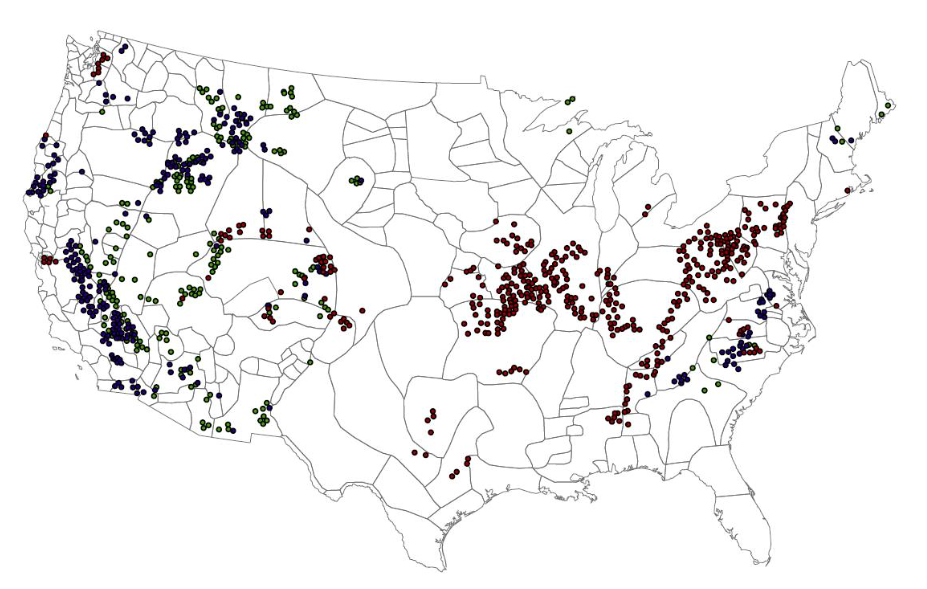
\includegraphics[scale=0.25]{mining.png}
    \caption{Geo-database on Mining Clusters in Precious Metals and Coal}
    \label{fig:strat:mining}
\end{subfigure}%
\begin{subfigure}{.5\textwidth}
    \centering
    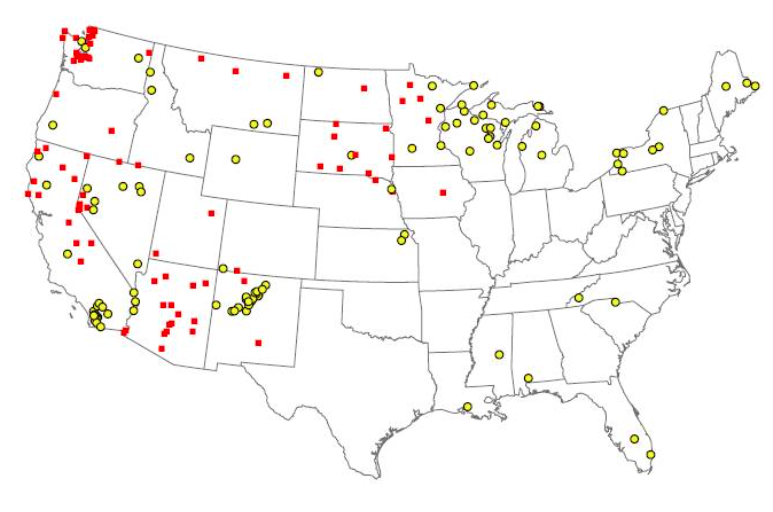
\includegraphics[scale=0.3]{forcedintegration.png}
    \caption{Reservations with (red square) and without (yellow circle) forced integration.}
    \label{fig:strat:reservations}
\end{subfigure}
\caption{Basis for stratifying by the presence of historical forced coexistence.}
\label{fig:strat}
\end{figure}

Thus, \cite{dippel2010forced} uses historical mining rushes in the western U.S. as an instrumental variable in the forced coexistence of Native American tribes.
The mining rushes, which are illustrated in Figure~\ref{fig:strat:mining}, serve as a source of exogenous variation which determines whether or not the government placed formerly hostile bands together onto reservations.
We do not perform this instrumental analysis ourselves and instead borrow data from Dippel on forced integration, which are illustrated in Figure~\ref{fig:strat:reservations}. 
Unfortunately, we therefore do not account for potential selection biases in forced integration which could have affected Dippel's earlier work, though the varying nature of Native American tribes in the West ameliorates much of this problem.
Due to historical forced migrations of eastern Native Americans to the West, such as the Trail of Tears, there are likely few characteristics which significantly affect health which are inherent in western Native Americans but are not found in eastern Native Americans besides forced coexistence.
% TODO rewrite this sentence

In our analysis we use the number of reservations in a state/region with and without forced coexistence.
This allows us to stratify data into two spatial camps: those data from states/regions where forced coexistence (FC) was likely and those data from states/regions where FC was less likely.
By comparing the health outcomes of Native Americans in these states over time, we separate and find the statistical effects of forced coexistence solely on health outcomes.
    
The overall effects of forced coexistence are somewhat complex, though the overall trend of health outcomes, even having separated out income, is clearly downward for Native Americans in FC regions. 
One of the ways we proxy for health outcomes is by comparing individuals' self-reported health statuses, which are either excellent, good, or fair/poor.
We find that individuals' perceptions of their own health are lower in FC regions. 
However, we find that the lion's share of this difference is caused by a fall in the percentage of people who report \emph{excellent} health and an increase in the share of those who report \emph{good} health.
That is, whether the region was subject to forced coexistence has little effect on the percentage of people that perceive they are of poor health. 
We theorize that much of this effect may stem from the relative nature of health perception, where individuals measure their health by looking at their neighbors, despite the overall health of the community being lower.

In more concrete results, we find that adult mortality per hundred thousand is higher in FC states, though the actual mechanism for this change is unclear because many of the important causes of death in FC communities did not feature a statistically significant change when compared to other Native American communities.

The policy implications of these findings are somewhat difficult to pinpoint.  
It would be highly costly to move Native American groups onto new reserves, so we first recommend further research into the diseases and other health conditions which are driving the gap in Native American health. 
We also recommend improving the delivery of healthcare, especially in the public sector within the reservations to try to make it ethnically blind. 
On the larger scale, we recommend further research into health outcomes in the Southern United States, where slavery and desegregation has created similar forced coexistence among formerly unequal or hostile groups.  


% % % % % % % % % % % % % % % %
% % % % % % % % % % % % % % % %
% % % % % % % % % % % % % % % %
% % % % % % % % % % % % % % % %
% % % % % % % % % % % % % % % %
% % % % % % % % % % % % % % % %
% % % % % % % % % % % % % % % %
% % % % % % % % % % % % % % % %
% % % % % % % % % % % % % % % %
% % % % % % % % % % % % % % % %
% 2 pages
\section{Literature}
%motivation, discuss 2-3 key articles, what are their shortcomings, what's left unanswered, external validity problems?
\cite{dippel2010forced} finds that forced integration lowers per capita incomes today by 30 percent. However, he does not look at what effect forced coexistence might have on health.

There are many studies on Native American health outcomes. 
\cite{levin2002geographic} show that the prevalence of cardiovascular disease is higher amongst tribes than in their surrounding states.
\cite{harwell2001cardiovascular} show that cardiovascular disease is more prevalent among American Indians than non-Indians.
\cite{patel2013health} writes about Native Americans perceive their diabetes.
\cite{beals2003racial} compare alcohol use in two reservations to national data.
\cite{may2005outcome} evaluate a public health approach to suicide prevention in a reservation.

There have also been a few studies that have explored the effects of political, geopolitical, historical, and economic factors on the prevelance and development of several prominent diseases, such as diabetes (\cite{patchell2014role}), pneumonia, tuberculosis, heart disease, and cancer (\cite{heiner2014demographic}).

There have been studies that explore health disparities.
\cite{mcguire2008new} analyze disparities in mental health and mental healthcare.
\cite{watson2006public} shows how federal sanitation interventions have reduced incidence of disease on Indian reservations and have been responsible for the convergence of Native American and White infant mortality.
\cite{jones2006persistence} details all of the etiologies that exist to try to explain the persistence of American Indian health disparities, and he argues that blaming incidence of disease on genetics is dangerous, as it reduces the obligation to intervene. More likely, disparities exist due to socio-economic inequality.

None of these consider the effect of forced integration on health outcomes.

% % % % % % % % % % % % % % % %
% % % % % % % % % % % % % % % %
% % % % % % % % % % % % % % % %
% % % % % % % % % % % % % % % %
% % % % % % % % % % % % % % % %
% % % % % % % % % % % % % % % %
% % % % % % % % % % % % % % % %
% % % % % % % % % % % % % % % %
% % % % % % % % % % % % % % % %
% % % % % % % % % % % % % % % %
% 1-2 pages
\section{Data}
The data come from the Center for Disease Control and Prevention (CDC). We use two separate data sets downloaded from the CDC's health interactive database.

\subsection{Adult mortality data}
The adult mortality data set contains the cause of death for Native Americans, and it is measured in deaths per 100,000.
The data set is segmented within the U.S. by state and by year 2000-2011 in 3 year segments.
The significant causes of death are cancer, diabetes, major cardiovascular diseases, heart diseases, Ischemic heart disease, heart attack, stroke, respiratory ailments, and liver disease and cirrhosis.

Table~\ref{sumstat} shows statistics for adult mortality per hundred thousand people, aggregated for all states.
The reason the number of observations varies for each disease is that diseases will be recorded as missing values in states where their mortality rates are too low.
The table also includes a column indicating whether the disease is chronic or not.

\begin{table}[htbp]\centering \caption{Summary statistics \label{sumstat}}
\begin{tabular}{l c c  c c}\hline\hline
\textbf{Variable} & \textbf{Mean} & \textbf{Std. Dev.} & \textbf{N} & \textbf{Chronic} \\\hline
all\_causes & 672.252 & 376.756  & 194 & No\\
cancer & 138.158 & 77.932  & 166 & Yes\\
diabetes & 59.31 & 30.74  & 86 & Yes\\
cardio & 209.017 & 111.124  & 180 & Yes\\
heart\_disease & 160.281 & 84.119  & 168 & Yes\\
ischemic & 111.663 & 63.896  & 151 & Yes\\
heart\_attack & 50.081 & 27.209  & 86 & No\\
stroke & 47.078 & 20.183  & 74 & No\\
respiratory & 50.982 & 29.281  & 73 & Yes\\
cirrhosis & 35.449 & 21.189  & 86 & Yes\\
\hline
\end{tabular}
\end{table}



\subsection{Self-reported health status data}
The first data set contains the self-reported health status for Native Americans, which is measured as excellent, good, or fair/poor, and it is measured in percent as well as base count.
The data take all of reported data from the Native American population of the U.S. and segments it by region of the country, by income status (poor, near poor, and non-poor) and by year from 1998-2012 in 3 year segments.

\subsubsection{Income hypothesis}
Figure~\ref{fig:health_status_by_income} shows the composition of self-reported health statuses across different income groups. Note that \emph{nonpoor}, the highest income group, has the largest percentage of people who reported they had ``excellent'' health and the smallest percentage of people who reported they had ``poor'' health. 
This is somewhat expected, as wealthier people tend to have better health. 
Wealthier people are on average more aware of their health and tend to report lower health statuses. 
However, we hypothesize that ``nonpoor'' people are reporting their health statuses relative to how they perceive the health of others. 

\begin{figure}[ht!]
\centering
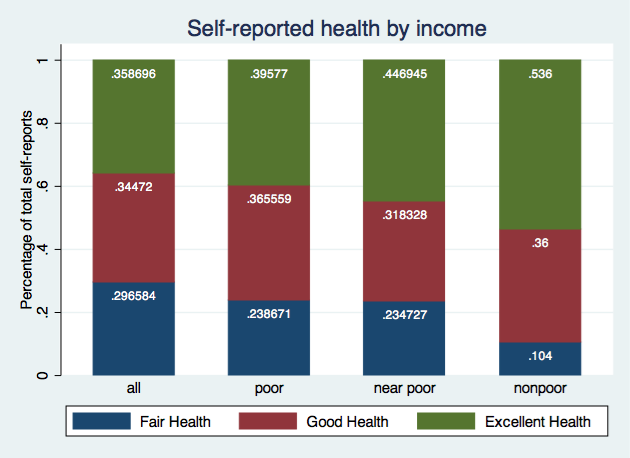
\includegraphics[scale=0.3]{health_status_by_income.png}
\caption{self-reported health by income}
\label{fig:health_status_by_income}
\end{figure}

\subsubsection{Region hypothesis}
Figure~\ref{fig:health_status_by_region} shows the composition of self-reported health statuses across different regions. 
Note that the northeast has the highest percentage of self-reported ``excellent''s and the lowest percentage of self-reported ``poor''s. 
The health status compositions of the Mountain and Pacific regions do not appear to be different from those of the Midwest and the South. 
However, we hypothesize that the Pacific and Mountain regions -- where there has been historical forced coexistence -- have a larger percentage of those who report poor health and a smaller percentage of those who report excellent health.

\begin{figure}[ht!]
\centering
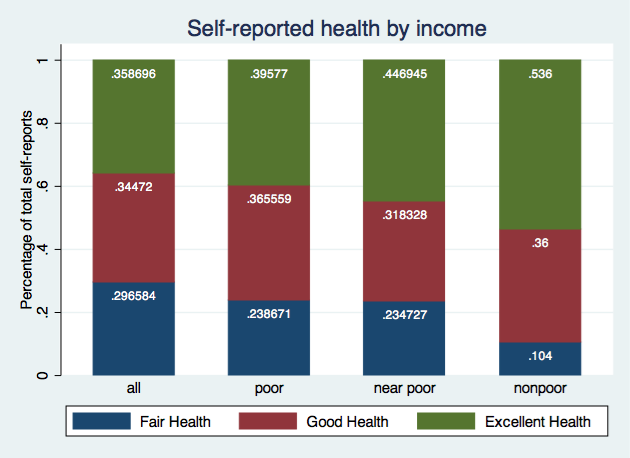
\includegraphics[scale=0.3]{health_status_by_income.png}
\caption{self-reported health by region}
\label{fig:health_status_by_region}
\end{figure}




% % % % % % % % % % % % % % % %
% % % % % % % % % % % % % % % %
% % % % % % % % % % % % % % % %
% % % % % % % % % % % % % % % %
% % % % % % % % % % % % % % % %
% % % % % % % % % % % % % % % %
% % % % % % % % % % % % % % % %
% % % % % % % % % % % % % % % %
% % % % % % % % % % % % % % % %
% % % % % % % % % % % % % % % %
\section{Results}

\subsection{What counts as a FC state/region?}
In order to execute our difference-in-differences strategy, we need to be able to separate regions and states into two camps: those that are likely to be FC and those that are less likely to be FC. For each state or region, we consider the ratio:
$$\frac{\mbox{\# of FC reservations}}{\mbox{\# of total reservations}}$$
We get both the numerator and the denominator from the location of both FC and non-FC reservations as seen in Figure~\ref{fig:strat:reservations}.

The states with the highest ratios are depicted in Table~\ref{fcpercent}.  From this data, we can see that Washington, Arizona, and South Dakota are the states with a significant number of reservations and with a high percentage of forced coexistence.

\begin{table}[ht!]
	\centering
    \begin{tabular}{ | l | l | l | l | }\hline\hline
    State        & \# FC & \# non-FC & Percentage FC \\\hline
	Iowa         & 1     & 0         & 100           \\
	Utah         & 2     & 0         & 100           \\
    South Dakota & 8     & 1         & 88.8          \\
	Washington   & 20    & 3         & 86.9          \\
    Arizona      & 15    & 3         & 83.3          \\
	Oregon       & 2     & 1         & 66.6          \\
    Montana      & 3     & 2         & 60            \\
    California   & 14    & 14        & 50            \\
    Nevada       & 6     & 6         & 50            \\
    North Dakota & 1     & 1         & 50            \\
    Minnesota    & 4     & 4         & 50            \\\hline
    \end{tabular}
    \caption{The extent to which states have historically forced sub-tribal bands to coexist.}
    \label{fcpercent}
\end{table}

\subsection{Adult mortality}
Table~\ref{fc1} shows that if a state is a FC state (Iowa, Utah, or South Dakota), then it is expected on average to have higher mortality for ``all causes.'' 
This reinforces the theory that forced integration has had a detrimental effect on Native American health outcomes. 
Moreover, the forced coexistence variable has a statistically significant effect on the mortality of diabetes and cirrhosis.
This is not the case, however, for other individual diseases, such as cancer, heart disease, and chronic respiratory diseases.

\begin{table}[htbp]\centering \caption{Effect of Forced Coexistence (IA, UT, SD) on Adult Mortality of Chronic Diseases\label{fc1}} \begin{tabular}{l*{8}{c}} \toprule
                    &\multicolumn{1}{c}{(1)}&\multicolumn{1}{c}{(2)}&\multicolumn{1}{c}{(3)}&\multicolumn{1}{c}{(4)}&\multicolumn{1}{c}{(5)}&\multicolumn{1}{c}{(6)}&\multicolumn{1}{c}{(7)}&\multicolumn{1}{c}{(8)}\\
                    &\multicolumn{1}{c}{all\_causes}&\multicolumn{1}{c}{cancer}&\multicolumn{1}{c}{diabetes}&\multicolumn{1}{c}{cardio}&\multicolumn{1}{c}{heart\_disease}&\multicolumn{1}{c}{ischemic}&\multicolumn{1}{c}{respiratory}&\multicolumn{1}{c}{cirrhosis}\\
\midrule
forced\_coex         &      1459.0&       153.1&       158.5&       333.1&       198.5&       74.54&       17.42&       75.67\\
                    &      (1.65)&      (0.81)&      (2.05)&      (1.26)&      (0.91)&      (0.48)&      (0.26)&      (1.49)\\
\addlinespace
Constant            &      2471.4&       440.7&       90.69&       718.1&       516.3&       326.2&       71.95&       55.32\\
                    &     (11.53)&      (9.57)&      (4.83)&     (11.22)&      (9.80)&      (8.63)&      (4.48)&      (4.49)\\
\midrule
Observations        &          51&          51&          51&          51&          51&          51&          51&          51\\
\bottomrule
\multicolumn{9}{l}{\footnotesize \textit{t} statistics in parentheses}\\
\end{tabular}
\end{table}


Table~\ref{fc2} shows the effect of forced coexistence on the mortalities of non-chronic diseases, such as stroke and heart attack. The FC effect is not significant on the mortality rates of either disease.
Moreover, according to Table~\ref{fc_chronic}, we lack the statistical power to show a significant relationship between a state being an FC state and its mortalities for both chronic and non-chronic diseases.

\begin{table}[htbp]\centering \caption{Effect of Forced Coexistence (IA, UT, SD) on Adult Mortality of Non-chronic Diseases\label{fc2}} \begin{tabular}{l*{2}{c}} \toprule
                    &\multicolumn{1}{c}{(1)}&\multicolumn{1}{c}{(2)}\\
                    &\multicolumn{1}{c}{heart\_attack}&\multicolumn{1}{c}{stroke}\\
\midrule
forced\_coex         &       93.02&       9.765\\
                    &      (1.43)&      (0.17)\\
\addlinespace
Constant            &       78.98&       67.74\\
                    &      (5.02)&      (4.83)\\
\midrule
Observations        &          51&          51\\
\bottomrule
\multicolumn{3}{l}{\footnotesize \textit{t} statistics in parentheses}\\
\end{tabular}
\end{table}

\begin{table}[htbp]\centering \caption{Effect of Forced Coexistence on Adult Mortality of (Non)Chronic Diseases\label{fc_chronic}} \begin{tabular}{l*{2}{c}} \toprule
                    &\multicolumn{1}{c}{(1)}&\multicolumn{1}{c}{(2)}\\
                    &\multicolumn{1}{c}{chronic}&\multicolumn{1}{c}{nonchronic}\\
\midrule
forced\_coex         &      1010.8&       102.8\\
                    &      (1.07)&      (0.88)\\
\addlinespace
Constant            &      2219.3&       146.7\\
                    &      (9.66)&      (5.16)\\
\midrule
Observations        &          51&          51\\
\bottomrule
\multicolumn{3}{l}{\footnotesize \textit{t} statistics in parentheses}\\
\end{tabular}
\end{table}





% % % % % % % % % % % % %
% % % % % % % % % % % % %
% % % % % % % % % % % % %
% % % % % % % % % % % % %
% % % % % % % % % % % % %
% % % % % % % % % % % % %
\subsection{Health status}
Originally there were three income levels: poor, nearpoor, and non-poor.
However, to simplify things, we consider \emph{nearpoor} as \emph{poor}, thereby giving us a convenient binary to work with.

\begin{table}[htbp]\centering \caption{Effect of Poor Income and Forced Coexistence on Health Statuses\label{poorfc}} \begin{tabular}{l*{6}{c}} \toprule
                    &\multicolumn{1}{c}{(1)}&\multicolumn{1}{c}{(2)}&\multicolumn{1}{c}{(3)}&\multicolumn{1}{c}{(4)}&\multicolumn{1}{c}{(5)}&\multicolumn{1}{c}{(6)}\\
                    &\multicolumn{1}{c}{\%\_excellent}&\multicolumn{1}{c}{\%\_good}&\multicolumn{1}{c}{\%\_fair}&\multicolumn{1}{c}{\%\_excellent}&\multicolumn{1}{c}{\%\_good}&\multicolumn{1}{c}{\%\_fair}\\
\midrule
forced\_coex         &      -8.632&       4.228&       3.281&            &            &            \\
                    &     (-6.47)&      (4.52)&      (2.18)&            &            &            \\
\addlinespace
income\_poor         &      -5.710&       2.829&       6.709&      -4.237&       2.461&       4.722\\
                    &     (-4.86)&      (3.15)&      (4.18)&     (-3.79)&      (2.96)&      (3.12)\\
\addlinespace
forced\_poor         &       1.369&       2.591&      -3.513&      -3.432&       3.433&       1.303\\
                    &      (0.73)&      (1.91)&     (-1.53)&     (-2.34)&      (3.17)&      (0.68)\\
\addlinespace
region\_p            &            &            &            &      -7.662&       5.835&      -2.621\\
                    &            &            &            &     (-6.08)&      (6.80)&     (-1.84)\\
\addlinespace
Constant            &       56.27&       30.15&       18.92&       54.79&       30.51&       20.91\\
                    &     (73.89)&     (54.06)&     (19.32)&     (82.36)&     (65.29)&     (25.65)\\
\midrule
Observations        &         568&         487&         356&         568&         487&         356\\
\bottomrule
\multicolumn{7}{l}{\footnotesize \textit{t} statistics in parentheses}\\
\end{tabular}
\end{table}


Table~\ref{poorfc} shows the effect of living in an FC region and being poor (or nearpoor) on all three levels of self-reported health statuses. It does this for two definitions of forced coexistence: one that include Pacific and Mountain regions, and one that only includes the Pacific.

Using both the Pacific and Mountain regions, we find that for all income groups, living in FC regions saw significantly lower levels of excellent health outcomes reported as well as an increased percentage stating their health to be merely good or fair among Native Americans.
Among the poor, who are especially populous among Native Americans, the interaction term between living in a FC region and being poor is statistically significant for percentage reporting good health, and it increases the percentage reporting good by 2.591 percentage points whereas income itself is statistically insignificant.
This suggests that forced coexistence plays a strong role in dropping self-reported health from excellent to good.

However, the interaction terms tell a slightly different story about the cause of these outcomes in potentially dropping health perception from good down to fair. 
In tables 2, 3, and 4 the interaction term on forced coexistence and wealth is not statistically significant with regards to fair self-reported health. 
This suggests that much of the differences seen in the forced coexistence term on percent of Native Americans reporting fair health are coming from differences in income or in other unexplained variables.  

In the Pacific, where the more speedy and haphazard forced integration occurred due to larger mining rushes, we see somewhat clearer negative results from forced coexistence. 
We see the same general results from region and income variables in worsening Native American health, but the interaction terms between forced coexistence and income are more significantly negative.  
Among the poor, the interaction variable between living in a FC state and poor income is statistically significantly dropping the percentage reporting excellent health by 3.912 percentage points and at the same time significantly increasing the percentage of people reporting good health by 5.145 percentage points.  
This is an even stronger effect than was seen in the combined Pacific and Mountain regions because most of the loss of excellent outcomes among the poor in the combined regions was due to income alone, not due to the combination of income and forced coexistence.

Again though, there is no statistically significant effect of the forced coexistence interaction term on any income group upon the fair outcomes, suggesting that forced coexistence is not drastically worsening poor Native Americans? health, but rather making it slightly worse, at least in their own perception. 

% % % % % %
\begin{table}[htbp]\centering \caption{Effect of Poor Income on Health Statuses in the Pacific and Mountain Regions\label{pmpoor}} \begin{tabular}{l*{3}{c}} \toprule
                    &\multicolumn{1}{c}{(1)}&\multicolumn{1}{c}{(2)}&\multicolumn{1}{c}{(3)}\\
                    &\multicolumn{1}{c}{percent\_excellent}&\multicolumn{1}{c}{percent\_good}&\multicolumn{1}{c}{percent\_fair}\\
\midrule
forced\_coex         &      -8.632&       4.228&       3.281\\
                    &     (-6.47)&      (4.52)&      (2.18)\\
\addlinespace
income\_poor         &      -5.710&       2.829&       6.709\\
                    &     (-4.86)&      (3.15)&      (4.18)\\
\addlinespace
forced\_poor         &       1.369&       2.591&      -3.513\\
                    &      (0.73)&      (1.91)&     (-1.53)\\
\addlinespace
Constant            &       56.27&       30.15&       18.92\\
                    &     (73.89)&     (54.06)&     (19.32)\\
\midrule
Observations        &         568&         487&         356\\
\bottomrule
\multicolumn{4}{l}{\footnotesize \textit{t} statistics in parentheses}\\
\end{tabular}
\end{table}

\begin{table}[htbp]\centering \caption{Effect of Poor Income on Health Statuses in the Pacific Region\label{ppoor}} \begin{tabular}{l*{3}{c}} \toprule
                    &\multicolumn{1}{c}{(1)}&\multicolumn{1}{c}{(2)}&\multicolumn{1}{c}{(3)}\\
                    &\multicolumn{1}{c}{percent\_excellent}&\multicolumn{1}{c}{percent\_good}&\multicolumn{1}{c}{percent\_fair}\\
\midrule
region\_p            &      -7.662&       5.835&      -2.621\\
                    &     (-6.08)&      (6.80)&     (-1.84)\\
\addlinespace
income\_poor         &      -4.237&       2.461&       4.722\\
                    &     (-3.79)&      (2.96)&      (3.12)\\
\addlinespace
forced\_poor         &      -3.432&       3.433&       1.303\\
                    &     (-2.34)&      (3.17)&      (0.68)\\
\addlinespace
Constant            &       54.79&       30.51&       20.91\\
                    &     (82.36)&     (65.29)&     (25.65)\\
\midrule
Observations        &         568&         487&         356\\
\bottomrule
\multicolumn{4}{l}{\footnotesize \textit{t} statistics in parentheses}\\
\end{tabular}
\end{table}


% % % % % % % % % % % % % % % %
% % % % % % % % % % % % % % % %
% % % % % % % % % % % % % % % %
% % % % % % % % % % % % % % % %
% % % % % % % % % % % % % % % %
% % % % % % % % % % % % % % % %
% % % % % % % % % % % % % % % %
% % % % % % % % % % % % % % % %
% % % % % % % % % % % % % % % %
% % % % % % % % % % % % % % % %
\section{Measurement issues}

Our data on self-reported health status is less precise than we would have liked because we were not able to find state by state income and health status data and were forced to use regions as a substitute.  This is a problem because state by state data is significantly more useful than regional data in evaluating the differences between FC and non-FC reservations because it has more statistical power.  Reservations in our FC states, Washington, South Dakota, and Arizona, are much more likely to have underwent forced coexistence than reservations in our FC regions, the Mountain and Pacific regions.

because the mountain and pacific regions are not as likely to have FC reservations and thus feature less statistical power than our state by state analysis of 

Similarly, we would have liked to include income data for our analysis of Native American mortality to  determine whether or not there was a significant interaction term between forced coexistence and income on this facted of Native American health.  This would have been an excellent robustness test for our analysis on the effects of FC which vary by income from our data on Native American self-reported health status.  

We are highly confident in the mortality figures as published by the CDC.  However, there is missing data for states for some diseases at given points in time due to their being too few deaths to estimate the true death rate per 100,000.

Beyond these specific issues, the analysis is somewhat weakened by the general measurement problems of self-reported health status and mortality.  Self-reported health status is greatly affected by the health of the individual's community, as the individual may be in poor health but sees himself as in good health in comparison to the people living near him.  Self-reported health status findings naturally lump around good, as people are likely to see themselves as in average health.  Moreover, poorer individuals are less likely to report themselves as being in poorer health due to lack of knowledge about their conditions, though this is dealt with in large part in our analysis by examining the interaction term between income and forced coexistence on health rather than simply the effects of forced coexistence.  

As for mortatlity, the CDC's data depends on institutional records which are imperfect, especially on Native American reservations, which could explain the significant prevalence of missing values in our CDC dataset.  However, there is no evidence that insitutional problems are more evident on FC reservations or that they affect the diseases we observe in a non-random manner, so it is reasonable to assume that these institutional problems do not significantly affect our analysis.


% % % % % % % % % % % % % % % %
% % % % % % % % % % % % % % % %
% % % % % % % % % % % % % % % %
% % % % % % % % % % % % % % % %
% % % % % % % % % % % % % % % %
% % % % % % % % % % % % % % % %
% % % % % % % % % % % % % % % %
% % % % % % % % % % % % % % % %
% % % % % % % % % % % % % % % %
% % % % % % % % % % % % % % % %
\section{Discussion}
\subsection{Self-reported health statuses}
\subsubsection{Interpreting the interaction term}
% TODO

\subsection{Adult mortality}
\subsubsection{The whole, but not the pieces}
Our forced coexistence dummy variable significantly explains on ``all causes'' but has no significance in explaining each individual cause (e.g., cancer, heart attack, stroke). 
This may be because there is insufficient statistical power to detect differences when split by the different diseases due to small changes (even if equivalent in percentage terms) whereas when they are aggregated there is not this problem. 
% TODO
% Are the coefficients consistent with the aggregate results? Also do the coefficients on the diseases add up to approximately the coefficient you  observe for all diseases?

% % % % % % % % % % % % % % % %
% % % % % % % % % % % % % % % %
% % % % % % % % % % % % % % % %
% % % % % % % % % % % % % % % %
% % % % % % % % % % % % % % % %
% % % % % % % % % % % % % % % %
% % % % % % % % % % % % % % % %
% % % % % % % % % % % % % % % %
% % % % % % % % % % % % % % % %
% % % % % % % % % % % % % % % %
\section{Conclusion}
To conclude, our main findings are that forced coexistence does have a significant effect on individuals? health outcomes, though not in the way that we imagined.  
Rather than decreasing perceptions of health across the board our findings reveal that most of the damage is done in reducing excellent health to more mediocre results.  
Moreover, we imagined that in terms of specific diseases, forced coexistence would have more of an effect in certain diseases, perhaps in ones with high contagiousness where social control would have to be exerted to keep the damages down.  
Instead, forced coexistence seemed to affect overall health conditions, like mortality, but did not have a statistically significant effect on any one cause of death.

This findings are important because they answer affirmatively that forced coexistence does effect health and because give us some valuable insight on how forced coexistence has damaged the Native American communities. 
The broad effects of forced coexistence suggest that health is being affected through overall less efficient administration of the reservation as compared to single nation Native American reservations.  
This could occur through mechanisms like lower overall income, worse delivery of public medical services, and uncertain reservation medical policies as Native American groups struggle politically. 
Also, though overall healthiness is damaged, it seems that it is fairly equitable among individuals in a society with forced coexistence, given that no diseases were more prominent and that Native Americans? perceptions of health were clumped heavily around good. 
They were in good health relative to their neighbors though they we?re likely lower than Native Americans in other reservations or off the reservation.  

Of course, further research is required in individual Native American reservations to pinpoint the true causes of these worse health outcomes. 
However, given what we now know, we recommend that policies be enacted to increase efficiency of health care delivery within the reservations of the Pacific and Mountain regions which experience forced coexistence. 
The exact nature of these programs will depend on the flaws discovered by more pinpointed research, but we expect there to be problems of insufficient information regarding diseases and distant or poorly stocked supply of medical services. 
These should be solved by providing subsidies for information and further provision of medicine in a cost effective manner. 
In addition to the policy implications, we believe this paper contributes to the literature on the long lasting health consequences of social strife and heavy handed government relocation of ethnic or racial groups.


\newpage
\bibliographystyle{te}
\bibliography{main}


\end{document}
